\documentclass[preview]{standalone}

\usepackage{amsmath}
\usepackage{amssymb}
\usepackage{stellar}
\usepackage{bettelini}
\usepackage{tikz}
\usepackage{fancybox}
\usepackage{makecell}

\usetikzlibrary{cd}

\hypersetup{
    colorlinks=true,
    linkcolor=black,
    urlcolor=blue,
    pdftitle={Stellar},
    pdfpagemode=FullScreen,
}

\begin{document}

\title{Stellar}
\id{storia-antico-regime}
\genpage

\begin{snippetdefinition}{antico-regime-definition}{Antico regime}
    Una società dominata dalla disuguaglianza e dall'ingiustizia.
    Antico regime è il termine con il quale gli storici indicano l'insieme delle istituzioni
    politiche, giuridiche, economiche e sociali caratteristiche di gran parte dell'Europa tra 16°
    e 18° secolo. L'espressione ancien régime (\quotes{antico regime}) fu introdotta dai rivoluzionari
    francesi del 1789 per contrapporre il vecchio regime prerivoluzionario al nuovo regime da
    loro creato in Francia con la Rivoluzione francese.
\end{snippetdefinition}

\begin{snippet}{antico-regime-caratteristiche}
    L'Antico regime era un tipo di società caratterizzata:
    \begin{itemize}
        \item dall'autorità di un sovrano assoluto alleato con un una Chiesa
            intollerante;
        \item dal diritto fondato sulle disuguaglianze di nascita, che non
            riconosceva il valore del merito e della competenza;
        \item da un ordinamento oppressivo che imponeva ai contadini le
            servitù personali e che in generale schiacciava i sudditi sotto il
            peso delle tasse.
    \end{itemize}

    L'antico regime è difficile da periodizzare perché è composto da diverse
    componenti di diverse epoche, anche di milleni di anni, ancora rigorosamente in vigore.
\end{snippet}

\section{Monarchia}

\begin{snippetdefinition}{monarchia-definition}{Monarchia}
    Forma di governo in cui i supremi poteri dello stato sono
    accentrati in una sola persona (re, sovrano, monarca), la cui carica non è elettiva e che può
    essere anche affiancata da altre istituzioni: m. \textit{Ereditaria}, \textit{non ereditaria}; m. \textit{Assoluta}, in
    cui il supremo governo statale è concentrato nel monarca; m. \textit{Limitata} o \textit{costituzionale},
    quando, accanto al monarca, vi sono altre istituzioni sovrane, quali il parlamento e il
    governo, che ne controllino il potere in base a una costituzione: si distingue
    la m. \textit{Costituzionale parlamentare} dalla m. \textit{Costituzionale pura} secondo che sia o no in
    vigore il principio parlamentare, ossia della necessità di un rapporto di fiducia fra
    esecutivo e legislativo.
\end{snippetdefinition}

\begin{snippet}{4eaa8b47-e9bd-45f7-b37d-e018de488593}
    Un uomo detenie quindi la sovranità, affidatagli generalmente da una divinità
    per guidare il popolo verso la prosperità (legittimazione divina del potere).
    La carica è ereditaria e a vita.
    Nelle monarchie assolute il potete è indivisibile, è tutto nelle mani
    della medesima persona.
\end{snippet}

\section{Repubblica}

\begin{snippetdefinition}{repubblica-definition}{Repubblica}
    Con riferimento all'età classica, al
    medioevo e alla prima età moderna, ogni stato non retto da un monarca o da un
    dittatore: la R. romana o di Roma, dal 509 al 31 a. C.; le r. oligarchiche della Grecia; le
    R. marinare italiane; la R. di Cromwell in Inghilterra (metà del sec. 17°), ecc. 
\end{snippetdefinition}

\begin{snippet}{3515258e-eca1-425c-9d2b-4d126fb86b22}
    Una parte dei cittadini detiene la sovranità, che viene esercitata entro i limiti stabiliti dalle leggi.
    Vi è una presenza di una pluralità di istituzioni.
    La carica pubblica non è ereditaria e generalmente limitata nel tempo.\\
    \textbf{\color{red}nota:} una repubblica non è necessariamente democratica.
\end{snippet}

\section{Impero}

\begin{snippetdefinition}{impero-definition}{Impero}
    Per impero si intende un organismo politico costituito da diversi paesi, popolazioni e Stati
    collocati anche in zone non contigue, in molti casi caratterizzato dalla presenza di razze
    diverse e culture e lingue non omogenee, ma sempre dotato di un centro politico e di un
    nucleo nazionale dominante che esercita sull'insieme il comando e il potere supremo.
    Nell'antichità e nel Medioevo a capo degli imperi vi erano i monarchi, mentre in età
    moderna e contemporanea imperi sono state anche alcune repubbliche.[…]
    Il maggiore e più durevole impero del mondo antico sorto in Occidente fu quello romano,
    le cui origini vanno ricondotte all'opera dell'imperatore Augusto a partire dal 27 a.C.: egli
    riordinò i grandi territori già conquistati da \href{http://www.treccani.it/enciclopedia/roma_(Enciclopedia_dei_ragazzi)/}{Roma} in età repubblicana, territori che
    sarebbero stati ulteriormente accresciuti dai suoi successori in Europa, Asia e Africa. I
    fondamenti della politica imperiale furono la superiorità militare dei Romani, una
    crescente uniformità amministrativa, la diffusione della cultura greco-latina come cultura
    egemone, l'allargamento della cittadinanza.\\
    Data la sua estensione, l'Impero venne diviso tra il 3° e il 4° secolo in una parte occidentale
    e in una parte orientale. Nel 4° secolo l'Impero divenne ufficialmente cristiano
    e \href{http://www.treccani.it/enciclopedia/costantino-i-il-grande_(Enciclopedia_dei_ragazzi)/}{Costantino} spostò la capitale principale da Roma a Costantinopoli. Nel 476 l'Impero
    d'Occidente crollò in seguito alle invasioni barbariche, mentre quello d'Oriente, l'\href{http://www.treccani.it/enciclopedia/impero-bizantino_(Enciclopedia_dei_ragazzi)/}{Impero bizantino},
    sopravvisse fino al 1453, quando venne definitivamente abbattuto dai Turchi
    ottomani.
\end{snippetdefinition}

\begin{snippet}{fdb8f561-02df-44aa-a1b6-c2052dda8f19}
    \begin{itemize}
        \item Generalmente comprende vasti territori e popoli diversi, soggetti ad un'unica autorità che garantisce l'equilibrio tra le varie componenti territoriali ed etniche;
        \item sono possibili modalità di nomina diverse per l'imperatore: elezione, designazione, ereditarietà;
        \item un impero si fonda su un'ideologia a carattere universale, ovvero ha l'ambizione di costruire l'unica civiltà esistente (o comunque una civiltà superiore).
    \end{itemize}
\end{snippet}

\section{Monarchia feudale}

\begin{snippetdefinition}{feudo-definition}{Feudo}
    Grossa proprietà terriera.
\end{snippetdefinition}

\begin{snippetdefinition}{monarchia-feudale-definition}{Monarhia feudale}
    Stato di proprietari, legati da un rapporto personale di subordinazione verso il sovrano che aveva donato loro la terra, e, con la terra, l'autorità.
\end{snippetdefinition}

\begin{snippet}{monarchia-feudale-potere-limitato}
    In una monarchia feudale il potere del sovrano è limitato:
    \begin{itemize}
        \item Non possiede una forza militare (diretta). La forza militare è quella dei feudatari che fanno giuramento verso il re;
        \item ha un potere fiscale ridotto;
        \item l'amministrazione del terrotorio e della giustizai è delegata ai signori, nobili feudatari, vassalli del re;
        \item il clero (la Chiesa) amministra le proprie terre;
        \item i comuni con status particolari (non sono sotto diretto potete del sovrano).
    \end{itemize}
\end{snippet}

\begin{snippetdefinition}{stato-definition}{Stato}
    Entità giuridica dotata del monopolio amministrativo,
    giudiziario, politico e coercitivo in un determinato
    territorio, coeso e munito di precise frontiere.
\end{snippetdefinition}

\plain{Lo stato è quindi un territorio con dei cittadini ed un governo.}

\begin{snippet}{caratteristiche-stato}
    Lo stato può essere:
    \begin{itemize}
        \item Autoritario (Es. Cina, Corea del Nord)
        \item Liberale/Democratico (Es. Svizzera)
        \item Unitario/Centralistico (Es. Italia, Monarchia che centra il potere)
        \item Federale (Es. Svizzera)
        \item Confederali (Es. ex Svizzera, Germania)
        \item Confessionale (Es. Vaticanow, Iran)
        \item Laico (non confessionale)
        \item Socialista (Es. Cina, Cuba, Corea del Nord)
        \item Capitalista
    \end{itemize}
\end{snippet}

\begin{snippetdefinition}{stato-moderno-definition}{Stato moderno}
    Lo \textit{stato moderno} è sorto in Europa
    tra il 15° e il 16° secolo, trovando la sua espressione dominante nella monarchia assoluta, che
    a partire dalle grandi monarchie nazionali di Spagna, Inghilterra e Francia pose gradualmente
    fine al particolarismo di matrice feudale o quanto meno lo ridusse fortemente ponendolo
    sotto il proprio controllo.
\end{snippetdefinition}

\begin{snippet}{50bb0cf1-92ae-4d39-9ba3-56b086a354b1}
    I suoi membri - individui e organismi collettivi - sono sottomessi unicamente alla legge,
    garanzia dei diritti statuiti e sottoposti al controllo dell'ordine giudiziario.

    Il primo tipo di stato è stato lo stato moderno, che poi si è trasformato in stato liberale democratico
    nei tempi moderni.
    Vi sono principalmente tre fattori che hanno procurato il passaggio da monarchia feudale a stato moderno:

    \begin{itemize}
        \item
        Il passaggio dal Medioevo al Rinascimento ha visto un profondo cambiamento nell'assolutismo, che non era più solo teorico ma divenne effettivo nel Cinquecento e Seicento. Questo cambiamento è attribuibile principalmente alla nuova struttura dello Stato, in particolare all'istituzione di eserciti permanenti che garantivano il potere del re. Questi eserciti, sia sotto forma di guarnigioni fisse che di truppe mobili, erano ora composti da fanterie mercenarie dipendenti solo dal re e non più dalla feudalità. La fanteria, diventata la principale forza militare, consentiva al sovrano di esercitare una politica estera più ampia.
        \item
        Inoltre, si è assistito a un cambiamento nella politica estera con l'organizzazione della prima diplomazia permanente, contrariamente al Medioevo in cui le relazioni internazionali erano meno strutturate. Questo cambiamento ha portato all'idea di equilibrio di potere tra gli Stati europei.
        \item
        Oltre all'esercito e alla diplomazia, la burocrazia statale è emersa come elemento chiave, con una crescente potenza degli "ufficiali"/funzionari del sovrano. In questo periodo, lo Stato si è concentrato attorno al potere sovrano e alla gerarchia degli ufficiali, piuttosto che sugli "ordini" della nazione o gli Stati generali.
        Vendita della cariche.
    \end{itemize}

    Questi processi mirano i ridurre il potere dei feudali ed aumentare quello del sovrano.

    Nel 1685 Luigi XIV comanda tutti gli Ugonotti di convertirsi al cristianesimo creando
    un'uniformità religiosa.

    Il Re diventato lo Stato sotto tutti gli effetti.
\end{snippet}

\section{La Società dell'Antico Regime}

\begin{snippet}{societa-antico-regime-illustration}
    \begin{center}
        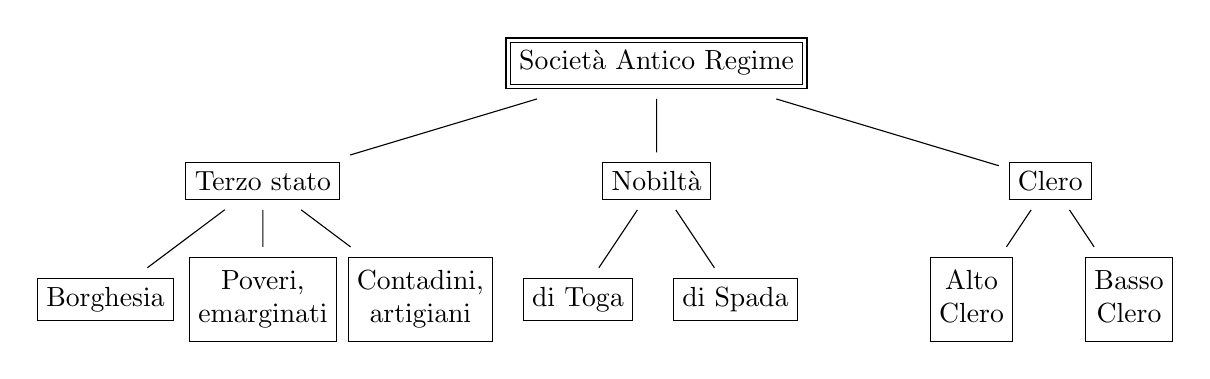
\begin{tikzpicture}[
            level 1/.style = {sibling distance = 5cm},
            level 2/.style = {sibling distance = 2cm}
        ]
        \node {\doublebox{Società Antico Regime}}
            child {
                node {\fbox{Terzo stato}}
                child {
                    node {\fbox{Borghesia}}
                }
                child {
                    node {\fbox{\makecell[c]{Poveri, \\ emarginati}}}
                }
                child {
                    node {\fbox{\makecell[c]{Contadini, \\ artigiani}}}
                }
            }
            child {
                node {\fbox{Nobiltà}}
                child {
                    node {\fbox{di Toga}}
                }
                child {
                    node {\fbox{di Spada}}
                }
            }
            child {
                node {\fbox{Clero}}
                child {
                    node {\fbox{\makecell[c]{Alto \\ Clero}}}
                }
                child {
                    node {\fbox{\makecell[c]{Basso \\ Clero}}}
                }
            };
        \end{tikzpicture}
    \end{center}
\end{snippet}

\begin{snippet}{f50405ec-b1b2-4853-b4a1-daf0d353a681}
    Non si può accedere al clero per nascita.
    Le tasse appartengono unicamente a quelli appartenenti al terzo stato.
    Non vi è libertà di pensiero, culto o parola.

    Questo tipo di società è divisa per discendenza eccetto per il Clero.
    Il primo genito di una famiglia nobiliare eredita spesso le varie terre, mentre il secondo genito
    andrà a fare parte dell'Alto Clero, mentre il Basso Clero è principalmente occupato dalla Borghesia.
\end{snippet}

\section{Fallimento dell'accentramento monarchico in Inghilterra}

\begin{snippet}{primo-sovrano-decapitato-antico-regime}
    Carlo I Stuart fu il primo sovrano decapitato dal popolo.
    Il parlamento in inghilterra non si fa scavalcare, e i sovrani, a differenza di quelli francesi,
    non riescono così tanto a centralizzare il potere.
    Il parlamento si ribella e obbliga i nuovi sovrani di firmare il \quotes{Bill of rights}.
\end{snippet}

\begin{snippetdefinition}{bill-of-rights-definition}{Bill of Rights}
    Il parlamento impone (non chiede) al sovrano di essere riconosciuto.
\end{snippetdefinition}

\begin{snippet}{25a8c8db-0800-465b-a2b8-8193b1ea6050}
    \begin{itemize}
        \item Il potere limtiato dal re;
        \item un parlamento rappresentativo dotato del monopolio legislativo;
        \item sistenza giudiziario a garanzia dell'integrità delle persone e di alcuni diritti indivuduali
    \end{itemize}
    
    Alcuni elementi per essere uno Stato moderno sono assenti, il potere non è infatti centralizzato.
    Tuttavia, è uno Stato Moderno perché riconosce i diritti individuali nei confronti del potere dello Stato.
    Seppur limitato, il otere del sovrano viene esercitato in modo uniforme su tutti i sudditi e su tutto il territorio.
    
    Il potere statuale non è più concentrato, bensì ripartito tra figure diverse:
    \begin{itemize}
        \item il re possiede il potere esecutivo;
        \item il parlamento ha potere legislativo;
        \item giudici hanno potere giudiziario.
    \end{itemize}
    
    % TODO stato liberale rappresentativo e le costituzioni
    % TODO differenza fra monarchia costituzionale e parlamentare
\end{snippet}

\section{Illuminismo}

\begin{snippetdefinition}{Illuminismo-definition}{Illuminismo}
    L'\textit{illuminismo} è una corrente di pensieri anche nominata l'età dei lumi.
    La luce alla quale si fa riferimento è in diretta contrapposizione
    al medioevo e diverse concezioni dell'Antico Regime, ossia, all'ignoranza.
\end{snippetdefinition}

\begin{snippet}{illuminismo-caratteristiche-expl}
    L'illuminismo è caratterizzato dall'autonomia dell'individuo e uso della ragione.
    Un movimento cosmopolita (La Natura, Il Cosmo sono gli stessi ovunque si metta piedei. Perciò essi
    potevano vivere allo stesso modo in accordo con la natura ovunque. Essi non erano a casa in una città
    o in un'altra, ma nella natura, nel Cosmo. Si chiamavano infatti cittadini del Cosmo: cosmopoliti).
    Inoltre, era caratterizato dalla tolleratanza; libertà di coscienza e di opinione.
\end{snippet}

% TODO def intolleranza. di alberto pincherie Encliclopedia italiana 1933

\plain{Possiamo cominciare a parlare di tolleranza quando vi sono motleplici religioni o teismi che sostengono di possedere la verità assoluta, le quali vanno in conflitto diretto con le altre.}

\begin{snippetdefinition}{giusnaturalismo-definition}{Giusnaturalismo}
    Il \textit{giusnaturalismo} è corrente filosofica giuridica, fondata su due principi:
    \begin{itemize}
        \item esiste un diritto naturale (conforme cioè alla natura dell'uomo e quindi intrinsecamente corretto);
        \item è superiore al diritto positivo (diritto prodotto dagli uomini).
    \end{itemize}
\end{snippetdefinition}

\begin{snippet}{03357b7f-ad6e-4633-81a4-7d336aca5686}
    Esistono norme di diritto naturale che hanno per oggetto la tutela della vita, della libertà e della proprietà.

    Nasce l'idea di avere un governo composto da 3 organi \textbf{separati}
    e \textbf{indipendenti} in maniera take che essi si bilancino e si frenino a vicenda.
\end{snippet}

\section{Voltaire}

\begin{snippetdefinition}{dispotismo-illuminato-definition}{Dispotismo illuminato}
    Il \text{dispotismo illuminato} è il governo assolutista di un monarca o despota illuminato.
\end{snippetdefinition}

\plain{Voltaire porta avanti il concetto di dispotismo assolutismo ma illuminato (intellettuali illuministri, consiglieri).
Il popolo va governato usando la ragione.}

\section{Rousseau}

\begin{snippet}{e27006e5-5af6-4257-9405-c403ca5eb376}
    Rousseau, mediante il \textit{Contratto Sociale} (1762),
    cercare di ridefinire il modo di vivere definendo una \textit{repubblica democratica}.
    Questo repubblica è di uguaglianza, tutti hanno gli stessi diritti degli altri.

    Piuttosto che prioritizzare l'individuo, si prioritizza collettivamente una meta comune
    che viene seguita con la \textit{volontà generale}.

    \begin{itemize}
        \item Gli uomini devono esercitare la libertà di fare le leggi (democrazia diretta);
        \item nel contratto sociale Rousseau ipotizza un patto in cui gli uomini non perdono mai la libertà nè la sovranità: questo patto è chiamato \textit{contratto sociale} e fonda la democrazia.
        \item senza il patto non c'è sovranità legittima;
        \item il patto fa entrare gli individui in una società politica: gli uomini si uniscono e nasce la volontà collettiva;
        \item gli uomini non si assoggettano, non cedono la sovranità a qualcuno, ma a sè stessi, ad un'assemblea di cittadini;
        \item nasce un io collettivo, comunità politica, nata in seguito ad un contratto.
    \end{itemize}
\end{snippet}

\section{La Dichiarazione di Indipendenza degli Stati Uniti (1776)}

\begin{snippet}{dichiarazione-indipendenza-expl}
    Il documento enuncia i principi dei diritti dell'uomo e della legittimità della rivoluzione,
    principi derivanti dall'illuminismo.
    Questi principi giustificano la rivoluzione e le colonie hanno quindi il diritto di
    diventare indipendenti dalla Gran Bretagna.
\end{snippet}

% TODO winner takes all
% la corte suprema si occupa di verificare che le leggi siano costituzionali
% può invalidare le leggi se rischia di essere anti costituzionale
% check and balance | controlla / veto

\section{Le rivoluzioni americana e francese}

\begin{snippet}{53080e77-ca60-4f17-bd75-a044cf5e7fd4}
    \begin{itemize}
        \item Una costituzione che limita il potere dello Stato con la divisione dei poteri.
        \item Una democrazia rappresentativa.
        \item Una potere repubblicano e/o monarchico costituzionale.
        \item Il riconoscimento dei diritti individuali e naturali dell'individuo.
    \end{itemize}
    
    Tutti sono uguali davanti alla legge, a differenza della società dell'Antico Regime,
    dove vi erano dei privilegi.
\end{snippet}

\section{La Dichiarazione dei diritti dell'uomo e del cittadino}

\begin{snippet}{dichiarazione-diritti-uomino-e-cittadino}
    \begin{enumerate}
        \item Gli uomini nascono e rimangono liberi e uguali nei diritti. Le distinzioni sociali
        non possono essere fondate che sull'utilità comune.
        \item Il fine di ogni associazione politica è la conservazione dei diritti naturali ed
        imprescrittibili dell'uomo. Questi diritti sono la libertà, la proprietà, la sicurezza e la
        resistenza all'oppressione.
        \item Il principio di ogni sovranità     risiede essenzialmente nella \textit{Nazione}.
        Nessun corpo o individuo può esercitare un'autorità che non emani espressamente da essa.
        \item La libertà consiste nel poter fare tutto ciò che non nuoce ad altri: così, l'esercizio
        dei diritti naturali di ciascun uomo ha come limiti solo quelli che assicurano agli altri
        membri della società il godimento di questi stessi diritti. Questi limiti possono essere
        determinati solo dalla Legge.
        \item  La legge ha il diritto di vietare solo le azioni nocive alla società. Tutto ciò che non
        è vietato dalla Legge non può essere impedito, e nessuno può essere costretto a fare ciò
        che essa non ordina.
        \item La Legge è l'espressione della volontà generale. Tutti i cittadini hanno il diritto di
        concorrere, personalmente o mediante i loro rappresentanti, alla sua formazione. Essa
        deve essere uguale per tutti, sia che protegga, sia che punisca. Tutti i cittadini essendo
        uguali ai suoi occhi sono ugualmente ammissibili a tutte le dignità, posti e impieghi
        pubblici secondo la loro capacità, e senza altra distinzione che quella delle loro virtù e
        dei loro talenti.
        \item Nessun uomo può esser accusato, arrestato o detenuto se non nei casi determinati
        dalla Legge, e secondo le forme da essa prescritte. Quelli che procurano, emettono,
        eseguono o fanno eseguire degli ordini arbitrari, devono essere puniti; ma ogni cittadino
        citato o tratto in arresto, in virtù della Legge, deve obbedire immediatamente;
        opponendo resistenza si rende colpevole.
        \item La Legge deve stabilire solo pene strettamente ed evidentemente necessarie e
        nessuno può essere punito se non in virtù di una legge stabilita e promulgata
        anteriormente al delitto, e legalmente applicata.
        \item Presumendosi innocente ogni uomo sino a quando non sia stato dichiarato
        colpevole, se si ritiene indispensabile arrestarlo, ogni rigore non necessario per
        assicurarsi della sua persona deve essere severamente represso dalla Legge.
        \item Nessuno deve essere molestato per le sue opinioni anche religiose, purché la
        manifestazione di esse non turbi l'ordine pubblico stabilito dalla Legge.
        \item La libera comunicazione dei pensieri e delle opinioni è uno dei diritti più preziosi
        dell'uomo; ogni cittadino può dunque parlare, scrivere, stampare liberamente, salvo
        rispondere all'abuso di questa libertà nei casi determinati dalla Legge.
        \item La garanzia dei diritti dell'uomo e del cittadino ha bisogno di una forza pubblica;
        questa forza è dunque istituita per il vantaggio di tutti e non per l'utilità particolare di
        coloro ai quali essa è affidata.
        \item Per il mantenimento della forza pubblica, e per le spese d'amministrazione, è
        indispensabile un contributo comune: esso deve essere ugualmente ripartito fra tutti i
        cittadini, in ragione delle loro sostanze.
        \item Tutti i cittadini hanno il diritto di constatare, da loro stessi o mediante i loro
        rappresentanti, la necessità del contributo pubblico, di approvarlo liberamente, di
        controllarne l'impiego e di determinarne la quantità, la ripartizione, la riscossione e la
        durata.
        \item La società ha il diritto di chieder conto a ogni agente pubblico della sua
        amministrazione
        \item Ogni società in cui la garanzia dei diritti non è assicurata, né la separazione dei
        poteri determinata, non ha costituzione.
        \item La proprietà essendo un diritto inviolabile e sacro, nessuno può esserne privato,
        salvo quando la necessità pubblica, legalmente constatata, lo esiga in maniera evidente,
        e previa una giusta indennità.
    \end{enumerate}
\end{snippet}

\begin{snippet}{90fb7063-b8e8-4334-9343-1b28b885bfd9}
    Il terzo articolo elimina ciò che è il potete divino all'interno della sovranità,
    e lo rimpiazza con solo ed unicamente il volere della nazione stessa.

    Il sesto articolo rompe la possibilità di acquistare o ereditare cariche di posizione.

    % Napoleone permette di esportare questi principi all'estero, fino in Svizzera.
\end{snippet}

\end{document}